\documentclass{report}

\usepackage[utf8]{inputenc}
\usepackage[T1]{fontenc}
\usepackage[francais]{babel}
\usepackage{hyperref} % Pour les liens
\usepackage{titlesec, blindtext}
\usepackage{microtype}
\usepackage{blindtext}
\usepackage{graphicx}
\usepackage[left=3cm,right=3cm,top=1cm,bottom=1.2cm]{geometry}
\graphicspath{{images/}}
\newcommand{\hsp}{\hspace{10pt}}
\titleformat{\chapter}[hang]{\Huge}{\thechapter{.}\hsp}{0pt}{\Huge}
\usepackage{listings} % pour code source
\usepackage{color}    % pour code source
\definecolor{mygreen}{rgb}{0,0.6,0}
\definecolor{mygray}{rgb}{0.5,0.5,0.5}
\definecolor{mymauve}{rgb}{0.58,0,0.82}
\lstset{ %
  backgroundcolor=\color{white},   % choose the background color; you must add \usepackage{color} or \usepackage{xcolor}
  basicstyle=\fontsize{10}{10}\selectfont,        % the size of the fonts that are used for the code
  breakatwhitespace=false,         % sets if automatic breaks should only happen at whitespace
  breaklines=true,                 % sets automatic line breaking
  captionpos=b,                    % sets the caption-position to bottom
  commentstyle=\color{mygreen},    % comment style
  frame=single,                    % adds a frame around the code
  keepspaces=true,                 % keeps spaces in text, useful for keeping indentation of code (possibly needs columns=flexible)
  keywordstyle=\color{blue},       % keyword style
  otherkeywords={*,...},            % if you want to add more keywords to the set
  escapeinside={(*}{*)},
  numbers=left,                    % where to put the line-numbers; possible values are (none, left, right)
  numbersep=5pt,                   % how far the line-numbers are from the code
  numberstyle=\tiny\color{mygray}, % the style that is used for the line-numbers
  rulecolor=\color{black},         % if not set, the frame-color may be changed on line-breaks within not-black text (e.g. comments (green here))
  showspaces=false,                % show spaces everywhere adding particular underscores; it overrides 'showstringspaces'
  showstringspaces=false,          % underline spaces within strings only
  showtabs=false,                  % show tabs within strings adding particular underscores
  stepnumber=2,                    % the step between two line-numbers. If it's 1, each line will be numbered.5
  stringstyle=\color{mymauve},     % string literal style
  tabsize=1,                       % sets default tabsize to 2 spaces
  title=\lstname,                   % show the filename of files included with \lstinputlisting; also try caption instead of title*
  language=bash                 % the language of the code
}

\title{%
    \begin{minipage}\linewidth
        \centering{
            RAPPORT DE PROJET \break
            "Cloud et virtualisation avec Openstack"
        }
    \end{minipage}
}
\author{%
    \begin{minipage}\linewidth
        \centering{Tutrice : BOUZIANE Hinde\break}
        \break
        \centering{
            Groupe : \break
            CULTY Alexandre,\break
            BENAIS Charles,\break
            BRESSAND Jérémy,\break
            ROGLIANO Théo
        }
        \break
    \end{minipage}
}
\date{2015 - 2016}

\begin{document}

\maketitle % Page de garde

\tableofcontents % Table des matières

\large % Pour la taille de la police

% ------------------------------ REMERCIEMENTS ------------------------------
\newpage
\chapter*{Remerciements}
    Nous tenons tout d'abord à remercier madame BOUZIANE Hinde, notre tutrice de projet, qui nous a permis de réaliser ce projet.\break

    Nous voulons aussi remercier l'équipe de Grid5000 qui nous à permis de réaliser ce projet sur leur système en nous donnant accès à leurs serveurs.


% ------------------------------ INTRODUCTION ------------------------------
\newpage
\chapter*{Introduction}
    \begin{quote}
        «Le cloud computing, c'est l'exploitation de la puissance de calcul ou de stockage de serveurs informatiques distants par l'intermédiaire d'un réseau.» [Wikipédia]
    \end{quote}
    \bigbreak

    %Dans les années 1950, les utilisateurs accédaient depuis leurs terminaux à leurs applications sur des serveurs appelés «mainframes», l'ancêtre du cloud computing.
    
    %Dans les années 2000, les ASP (fournisseur de service d'application), apparaissent et hébergent des serveurs web, mails, etc.
    
    Le cloud est né à la suite de la multiplication des centres de données, de l'expension de la vitesse des communications et de la vitesse des calculs ainsi que de la maitrise de la virtualisation.\bigbreak

    L'intérêt du cloud tiens dans le fait que les serveurs sont loués à la demande, et que la facturation soit fait à l'usage. Autrement dit, le client paye uniquement l'utilisation réelle qu'il en a fait, pour les caractéristiques précises qu'il peut modifier.\bigbreak
    
    Avec le cloud computing plus besoin de serveurs locaux à entretenir, tous les services sont accessible via Internet et sont interconnectés.\bigbreak
    
    On distingue trois grands services de cloud :
    \begin{itemize}
        \item IaaS : Infrastructure as a Service, qui donne accès à des machines virtuelles ( que nous appelerons par la suite des VM ) sur lesquelles l'utilisateur peut installer son propre système d'exploitation et faire évoluer les caractéristiques du serveur à la demande (exemple : location d'un VPS).
        \item PaaS : Platform as a Service, l'utilisateur installe ses propres applications (exemple : installation de LAMP).
        \item SaaS : Software as a Service, les applications sont directement mis à disposition des utilisateurs, celui-ci ne s'occupe en rien de la gestion du serveur (exemple : utilisation d'un logiciel de VoIP).
    \end{itemize}
    \bigbreak
    \begin{figure}
        \includegraphics[width=\textwidth]{responsabilites}
        \caption{Les responsabilités par service du cloud [Wikipédia]}
    \end{figure}   
    
   %Il existe aussi d'autres services, comme par exemple le DaaS (Data as a service), STaaS (Storage as a service), etc, mais les trois cités plus haut sont les plus populaires.\break
     
    OpenStack est un logiciel composé d'un ensemble de modules permettant l'orchestration et le monitoring d'un cloud. Il fait partie de la catégorie des IaaS.\bigbreak
    
    \begin{figure}
        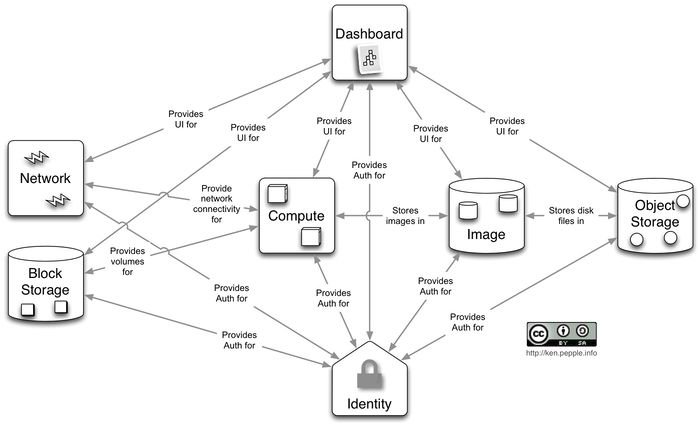
\includegraphics[width=\textwidth]{openstack_arch}
        \caption{Les responsabilités par service du cloud [Wikipédia]}
    \end{figure}
    
    Les 5 principaux modules sont Horizon, Nova, Neutron, Glance, Keystone:
    \begin{itemize}
        \item Glance est le gestionnaire d'image, il permet la découverte, l'envoi et la distribution d'image disque vers les instances. Les images stockées font office de modèle de disque.
        \item  Keystone est le service d'identité, il fournit un annuaire central contenant la liste des services et la liste des utilisateurs d'Openstack ainsi que leurs rôles et autorisations.
        \item  Horizon est le tableau de bord d'OpenStack.
        \item  Neutron permet de gérer et manipuler les réseaux et l'adressage IP au sein d'OpenStack.
        \item  Enfin Nova est le module que nous avons le plus manipulé, son but est de gérer les ressources de calcul des infrastructures. Nous comptons l'utiliser pour fournir un SaaS à l'utilisateur de notre application. 
    \end{itemize}
    \bigbreak
    %Voir le schéma wikipédia des modules
    %L'une des composantes d'OpenStack, appellée Swift, un système de stockage d'objets que nous n'avons pas utilisé pour notre projet.\bigbreak
    
    L'objectif de ce projet est de prendre en main les principes de bases de la virtualisation et du cloud computing à travers OpenStack, en particulier l'orchestration.\bigbreak
    
    Nous présenterons , dans un premier temps le travail effectué, puis les problèmes que nous avons rencontrés.\bigbreak
    
    
% ------------------------------ CONTENU ------------------------------
% --------------- 1 ---------------
\newpage
\chapter{Domaines d'applications}

    \section{Virtualisation}
        \subsection{Ressources}
            Attribuer une taille à une VM (mémoire vive, stockage, architecture)
        \subsection{Sauvegarde des données}
            Les VM ne sont pas immortelles, ils faut sauvegarder les resultats de nos app dans des block de données ou des fichiers.
            
    \section{Multiprocessing}
        \subsection{Creation processus application vm}
            Pour l'installation et le lancement d'application sur une VM, on lui détache un processus.
        \subsection{Processus en arrière plan/premier plan}
            Attacher/dettacher des screen ?
        \subsection{Communication inter processus}
            Screen ?
            
    \section{Reseau}
        \subsection{Configuration réseau déjà existant}
            Definir/créer les adresses ip flottantes, ouvrir les ports.
        \subsection{Creation réseau}
            Heat ?
        \subsection{communication entre VM}
            Serveur client perroquet, chat
        \subsection{navigation}
            SSH SCP
            
    \section{Systeme}
        \subsection{Pattern matching}
            expressions régulières.. 
            
    \section{Application}
        \subsection{Parametrage}
                Afin de passer beaucoup de paramètre de manière structurée à notre script, on créé un fichier utilisateur json.
        \subsection{Généralisation}
                Notre script doit etre capable d'installer et de lancer n'importe quelle application sur un ensemble de VM, ce qui implique
                l'utilisation d'un grand nombre de variables et des boucles et des structures de controle.
        \subsection{Partir des applications vers les VM}
                L'utilisateur ne doit pas se soucier des VMs, il se soucie seulement de son application. En gros on cache les aspects techniques au client.\break
        



%Expliquer ici openstack ou du moins mettre le schéma frontend/controller/serveur et VM (reprendre celui du dashboard)



% --------------- 2 ---------------
\chapter{Travail réalisé}
    \section{Mise en place}
        \subsection{DevStack}
            Dans le but de nous familiariser avec ce nouvel environnement,
            et l'accès à des machines possédant les droits administrateurs (sudo)
            ne nous étant pas offert à la faculté des sciences,
            nous avons choisi de mettre en place OpenStack sur nos machines personnelles.\break
            Devstack est un script bash automatisant la mise en place des modules OpenStack.

        \subsection{Grid5000}
        
            Tout d'abord, nous avons commencé par le tutoriel getting started qui nous a appris les règles d'utilisation,  les réservations de jobs et l'architecture de grid5000.  (https://www.grid5000.fr/mediawiki/index.php/Getting_Started)
            
            Ensuite, nous avons suivi le tutoriel "OpenStack deployment on Grid5000".  (https://www.grid5000.fr/mediawiki/index.php/OpenStack_deployment_on_Grid5000 )
        
        
            Dans un second temps il nous à été offert l'opportunité de travailler sur les clusters
            de Grid5000, un Réseau de Ressources distribuées supporté par l'INRIA et le CNRS.\break
            
            Cela nous a permis de comprendre grâce au tutoriel
            les différentes étapes de l'installation d'openstack, ainsi que les commandes de base pour son utilisation.
            Nous avons lancé les commandes suivantes afin de créer plusieurs VM, de copier des fichiers dans les VM, d'exécuter des petits programmes et tester le réseau
            en essayant de ping une VM depuis une autre VM.
            \lstinputlisting[language=bash, firstline=3, lastline=9, caption=Premier script : connection grid5000 et téléchargement xp5k-openstack]{./script1.sh}
            \lstinputlisting[language=bash, firstline=16, lastline=22, caption=Premier script : Création fichier configuration xp.conf]{./script1.sh}
            \lstinputlisting[language=bash, firstline=25, lastline=26, caption=Premier script : Démarrage d'une nouvelle "fenetre" et lancement openstack]{./script1.sh}
            \lstinputlisting[language=bash, firstline=30, lastline=30, caption=Premier script : Copie clé ssh publique sur le frontend]{./script1.sh}
            \lstinputlisting[language=bash, firstline=32, lastline=36, caption=Premier script : Connection au controlleur plus creation VM et IP publique]{./script1.sh}
            \lstinputlisting[language=bash, firstline=40, lastline=42, caption=Premier script : Attribution de l'IP à la VM et connection à la VM]{./script1.sh}
            \lstinputlisting[language=bash, firstline=48, lastline=48, caption=Premier script : Copie d'un fichier du frontend vers la VM]{./script1.sh}
            \lstinputlisting[language=bash, firstline=52, lastline=52, caption=Premier script : Execution d'une commande bash sur l'ensemble des VM]{./script1.sh}
            
            
    \section{Nos premiers scripts}
        \subsection{Automatiser installation application}
            \lstinputlisting[language=bash, firstline=8 lastline=8, caption=Installateur d'application : On récupère l'adresse du controlleur]{./APP_installer.sh}
            \lstinputlisting[language=bash, firstline=12 lastline=12, caption=Installateur d'application : On se connecte au controlleur et on récupère les adresses ip des VM]{./APP_installer.sh}
            \lstinputlisting[language=bash, firstline=18 lastline=20, caption=Installateur d'application : On se connecte a une VM et on installe l'application]{./APP_installer.sh}
        \subsection{Automatiser creation VM}
            \lstinputlisting[language=bash, firstline=1, lastline=50, caption=VM launcher]{./VM_launcher.sh}
        \subsection{Automatiser le deploiement d'openstack sur grid5000}
            \lstinputlisting[language=bash, firstline=12, lastline=13, caption=Deploiement : On recupère le login et le site]{./deploiement.sh}
            \lstinputlisting[language=bash, firstline=18, lastline=18, caption=Deploiement : On copie les fichier de l'app vers le frontend]{./deploiement.sh}
            \lstinputlisting[language=bash, firstline=26, lastline=27, caption=Deploiement : On se connecte au site]{./deploiement.sh}
            \lstinputlisting[language=bash, firstline=56, lastline=56, caption=Deploiement : On lance l'installation d'openstack]{./deploiement.sh}
            
    \section{Nos scripts tout en 1}
        \subsection{Premier gros script}
            
    \begin{figure}[!h]
        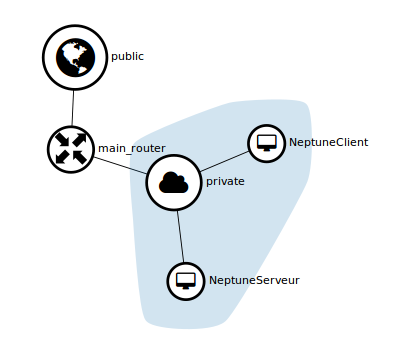
\includegraphics[width=\textwidth]{network-topo}
        \caption{Topologie du Network}
    \end{figure}

% --------------- 3 ---------------
\chapter{Problèmes rencontrés}
    \section{DevStack}
        Les premières semaines du TER, nous avons commencer par travailler OpenStack en utilisant DevStack, 
        qui permet d'installer différents modules de base OpenStack sur une unique machine.\bigbreak
        \subsection{Installation et configuration}
            DevStack requiert une configuration minimale, ainsi que des prérequis de configuration (systeme, network).\bigbreak
            Il n'à pas été aisé de mettre en place cette configuration, et, quand bien même une configuration 
            DevStack ait été correctement mise en place et fonctionnelle, celle-ci n'à pour durée de vie qu'une session !\bigbreak

    \section{OpenStack sur Grid5000}
        Chacun rencontrant des difficultés lors du déploiement DevStack Mme. BOUZIANE à pu obtenir un accès au reseau 
        de Grid5000 afin de pouvoir utiliser les scénarios de déploiement d'OpenStack existants.\bigbreak
        \subsection{Découverte}
            Tout d'abord même si celà n'a pas vraiment été un problème mais plutôt une étape nécessaire, nous avons dû comprendre comment le déploiement d'Openstack s'opère et les nouveaux outils mis à notre disposition (comme la commande rake).\bigbreak
        \subsection{Choix des languages}
            Voulant écrire des scripts, nous nous sommes naturellement orientés vers le language Bash. Nous nous sommes vite rendu compte que celà n'eut pas été le choix le plus judicieux de par la pénibilité syntaxique et les limitations du language. C'est une des raisons qui nous a poussé à passer progressivement à des scripts en ruby. L'autre raison étant que xp5k est en partie écrit en ruby.\bigbreak
        \subsection{Récupération de variable et flux}
            Lors de nos scripts nous accédons à de nombreuses machines et, notamment, entrons et sortons de nombreuses fois dans notre "controller". Nous avons d'abord utiliser la commande rake (effet de découverte) puis nous nous sommes vite appuyé sur ssh pour pouvoir récupérer des résultats ou des varibles d'environnement via des flux (pipe).\bigbreak
            
            De plus, nous n'avons pu récupérer certaines informations sans devoir les faire afficher dans le terminal et les récupérer par une regexp. Celà est une voie d'amélioration future.\bigbreak
            %Etoffer avec problemes SSH%
            
        \subsection{Copie de fichier}
            Une des difficultés pour l'écriture des scripts est le fait qu'ils nous aient impossible de copier un fichier exterieur à grid5000 vers grid5000 en étant au sein de celui ci. Nous sommes donc partis du principe qu'en prérequis le client copie les fichiers de son laptop vers grid5000.\bigbreak
        
        \subsection{IDE}
            Conséquence de la difficultée précédente, vu qu'il est peu aisé de copier des fichiers vers grid5000 en permanence, nous utilisons les éditeurs de textes (vim et nano) mis à notre dispostion sur le cluster pour des petites modifications lors des phases de tests. Malheuresement, ceux-ci sont assez peu ergonomique et plutôt contraignant sur la durée.\bigbreak
            
        \subsection{Automatisation de lancement d'une application}
            Pour lancer une application automatiquement
            
        \subsection{XP5K-OpenStack}
            %Blah
% ------------------------------ CONCLUSION ------------------------------
\newpage
\chapter*{Conclusion}
 

% ------------------------------ RESSOURCES DOCUMENTAIRES ------------------------------
\newpage
\chapter*{Ressources documentaires}
\href{http://docs.openstack.org/developer/devstack/}{Devstack} :
\url{http://docs.openstack.org/developer/devstack/}
\bigbreak
\href{http://www.openstack.org/}{Openstack} :
\url{http://www.openstack.org/}
\bigbreak
\href{https://www.grid5000.fr/}{Grid5000} :
\url{https://www.grid5000.fr/}
\bigbreak
\href{https://fr.wikipedia.org/wiki/Cloud_computing/}{Wikipédia} :
\url{https://fr.wikipedia.org/wiki/Cloud_computing/}



% ------------------------------ ANNEXES ------------------------------
\newpage
\chapter*{Annexes}


\end{document}
% --------------------------- INSTALLATION LATEX ----------------------
%sudo apt-get install texlive
%sudo apt-get install texlive-lang-french
%sudo apt-get install texlive-latex-extra
% Compile Time : pdflatex Rapport.tex
% Pensez à virer les .log, .aux, .out ET .pdf avant de push !
